\section{Results}

We evaluated decoding performance using the root mean squared error (RMSE) of the reconstructed trajectories, together with runtime and the competition score. Table~\ref{tab:hard_decoder} summarises representative results from the Hard Direction Decoder, while Table~\ref{tab:pca_decoder} reports the performance of the proposed Time-Dependent PCA Decoder.

\begin{table}[htbp]
\centering
\caption{Performance of the Hard Direction Decoder (representative variants).}
\label{tab:hard_decoder}
\begin{tabular}{lccc}
\hline
Method & RMSE & Time (s) & Score \\
\hline
Template + Ridge + Integration & 21.82 & 1.57 & 19.79 \\
Template + PCA + Ridge + Kalman & 21.09 & 1.85 & 19.17 \\
SVM + Ridge + Kalman & 22.28 & 3.59 & 20.41 \\
SVM + Ridge + learned CA-KF & 22.09 & 2.61 & 20.14 \\
\hline
\end{tabular}
\end{table}

Within the Hard Direction Decoder, improvements such as PCA-based denoising, alternative classifiers (e.g., SVM), and refined Kalman filtering resulted in only modest performance gains, with RMSE remaining around 21--23.

\begin{table}[htbp]
\centering
\caption{Performance of the Time-Dependent PCA Decoder.}
\label{tab:pca_decoder}
\begin{tabular}{lccc}
\hline
Method & RMSE & Time (s) & Score \\
\hline
Baseline time-dependent model & 8.03 & 3.44 & 7.57 \\
+ soft direction blending & 7.83 & 3.42 & 7.38 \\
Final model (tuned PCA + smoothing) & \textbf{7.50} & 3.17 & \textbf{7.07} \\
\hline
\end{tabular}
\end{table}

In contrast, the proposed Time-Dependent PCA Decoder achieved a substantially lower RMSE of approximately 7.5, representing a significant improvement over the Hard Direction Decoder. This indicates that redesigning the decoding pipeline is more effective than refining individual components within a fixed structure.\\

The performance gain can be attributed to three main factors. First, PCA-based low-dimensional representations provide a compact and noise-robust description of neural activity. Second, direction inference in this reduced space improves reliability compared to early hard decisions. Third, soft blending of multiple candidate directions and lightweight causal stabilisation reduce sensitivity to early decoding errors and improve temporal consistency.


\begin{figure}[htbp]
\centerline{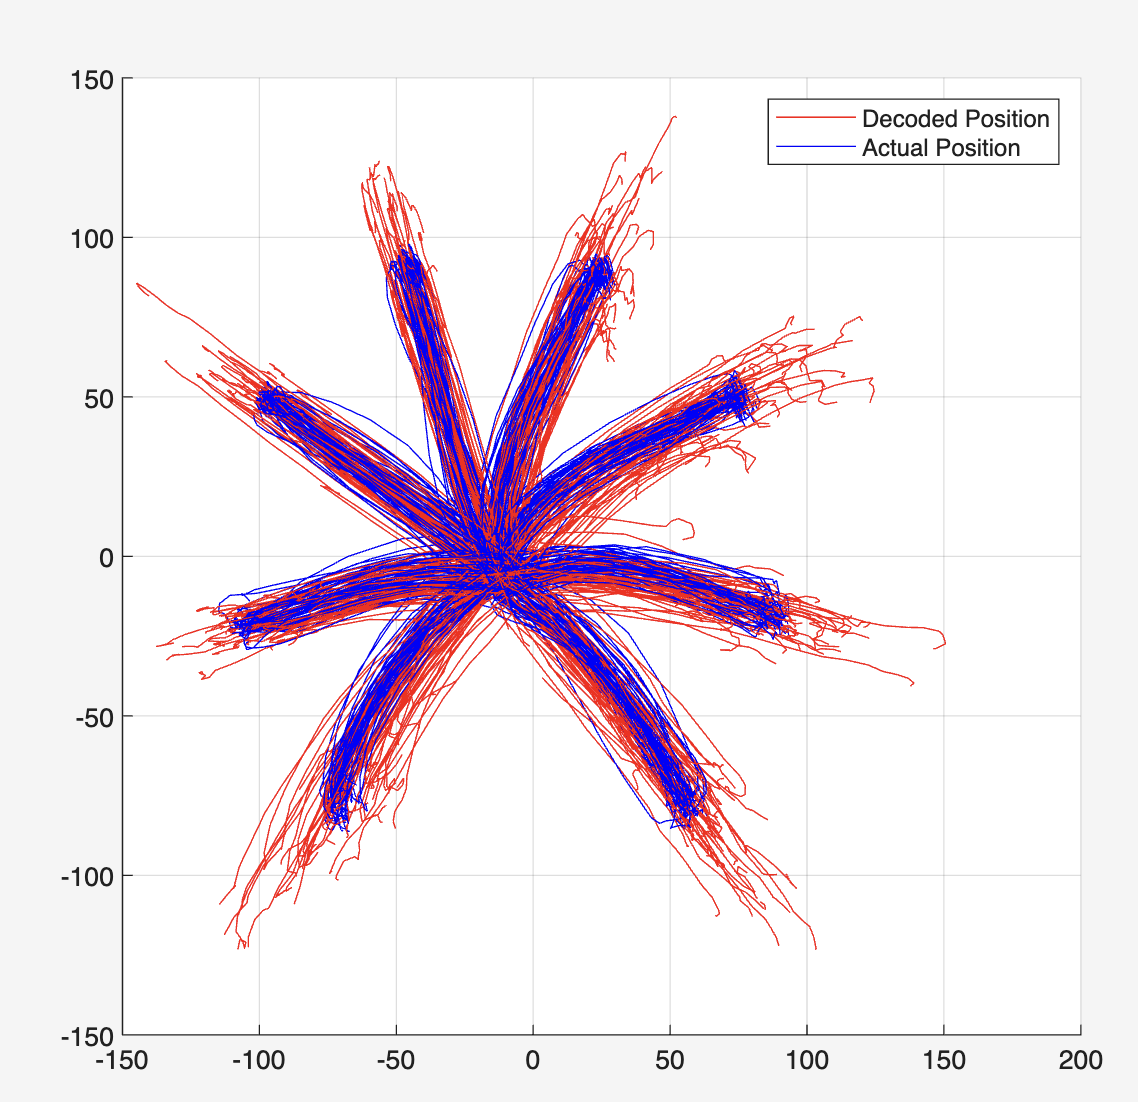
\includegraphics[width=0.85\columnwidth]{results/hand-position-estimation-using-hard-direction-decoder-v1.png}}
\caption{Decoded trajectories (red) versus ground truth (blue) using the Hard Direction Decoder. The decoded paths capture the general reaching directions, but show larger deviations and greater trajectory spread, reflecting sensitivity to early hard direction selection and accumulated estimation error.}
\label{fig:hard_trajectory}
\end{figure}

\begin{figure}[htbp]
\centerline{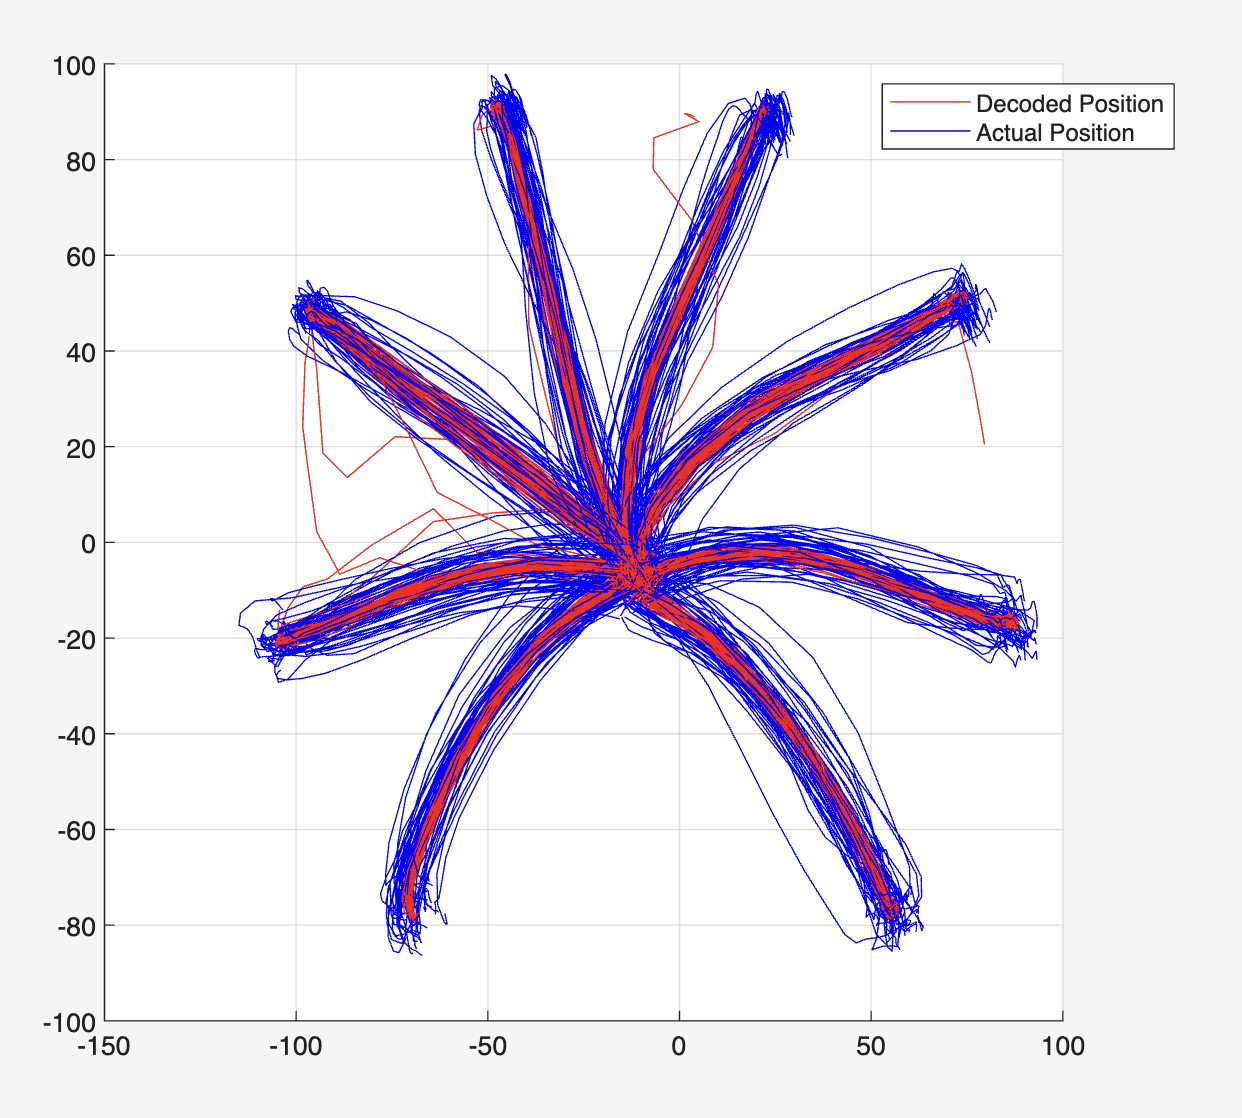
\includegraphics[width=0.85\columnwidth]{results/hand-position-estimation-using-time-dependent-pca-decoder-v5.png}}
\caption{Decoded trajectories (red) versus ground truth (blue) using the Time-Dependent PCA Decoder. Compared with the Hard Direction Decoder, the decoded trajectories are more tightly aligned with the true movements and show smoother behaviour across reaching directions.}
\label{fig:pca_trajectory}
\end{figure}

Figure~\ref{fig:hard_trajectory} shows that the Hard Direction Decoder captures the overall radial structure of the reaching task, but produces visibly larger deviations from the true trajectories. In contrast, Fig.~\ref{fig:pca_trajectory} shows that the Time-Dependent PCA Decoder generates trajectories that are more tightly aligned with the ground truth, consistent with its lower RMSE.

Figure~\ref{fig:pca_trajectory} illustrates representative decoded trajectories. The proposed method closely follows the ground truth across all reaching directions, while maintaining smooth and consistent trajectories over time.


Overall, these results demonstrate that appropriate use of low-dimensional structure and pipeline design leads to substantial improvements in decoding accuracy, while remaining fully causal and computationally efficient.

\begin{figure}[htbp]
\centerline{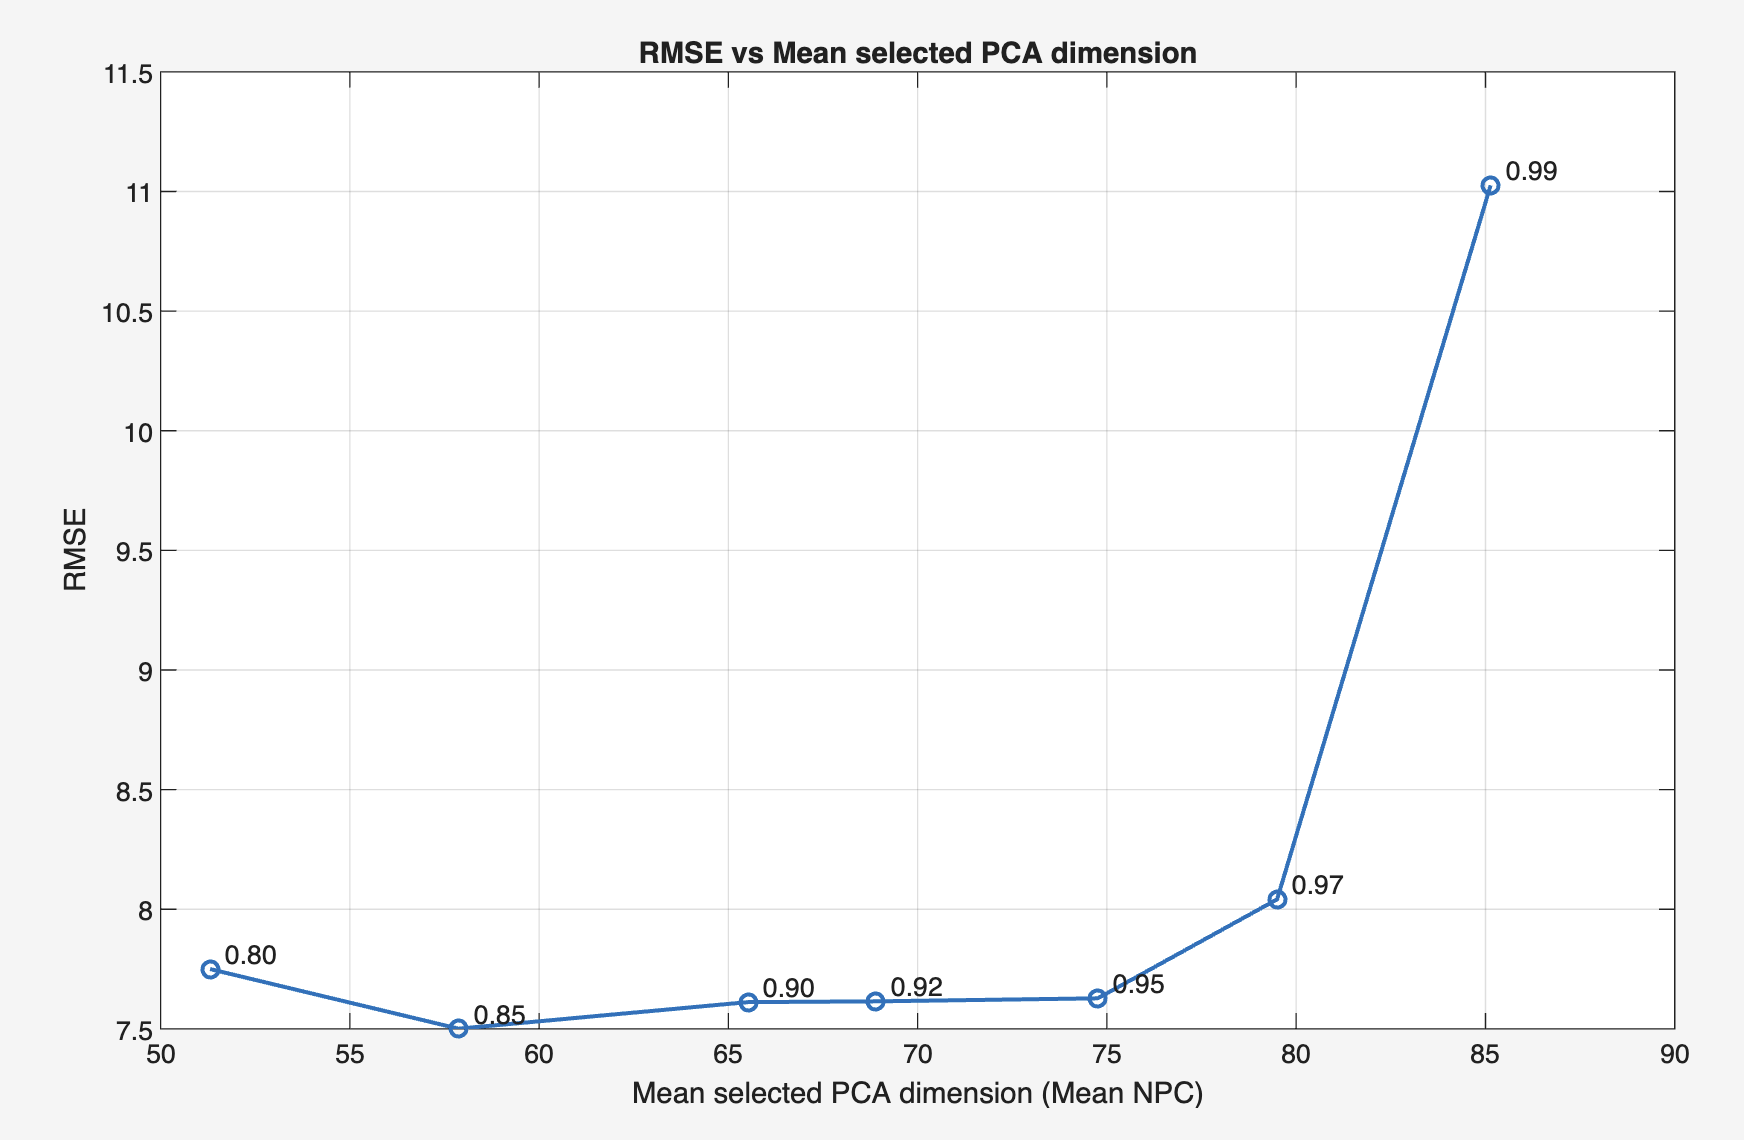
\includegraphics[width=0.95\columnwidth]{results/RMSE-vs-Mean-Selected-PCA-Dimension-v5.png}}
\caption{RMSE as a function of the mean number of selected PCA dimensions. Each point corresponds to a different variance retention threshold. An intermediate dimensionality achieves the best performance, while too few or too many components lead to increased error.}
\label{fig:pca_dimension}
\end{figure}

We further analysed the effect of PCA dimensionality on decoding performance (Fig.~\ref{fig:pca_dimension}). The results show a non-monotonic relationship between the number of retained principal components and RMSE.

Best performance is achieved at an intermediate dimensionality, corresponding to a variance retention of approximately 0.85. When too few components are retained, important task-relevant information is lost. In contrast, retaining too many components introduces noise and degrades performance.

This result highlights the importance of balancing information preservation and noise suppression when constructing low-dimensional neural representations.